% ===============================================================================
% ゼミ発表用スライド:一般化ペアワイズ比較における代入法の比較研究
% Overleaf完全対応版(日本語表示保証)
% ===============================================================================

\documentclass[11pt,aspectratio=169]{beamer}

% テーマとカラー設定
\usetheme{Madrid}
\usecolortheme{default}

% 日本語対応(Overleaf推奨設定)
\usepackage{xeCJK}
\setCJKmainfont{Noto Sans CJK JP}

% 代替設定(上記が使えない場合)
% \usepackage{luatexja}
% \usepackage[no-math]{luatexja-fontspec}

% パッケージ
\usepackage{amsmath, amssymb}
\usepackage{graphicx}
\usepackage{booktabs}
\usepackage{array}
\usepackage{tikz}
\usepackage{pgfplots}
\usepackage{xcolor}
\usepackage{hyperref}

\pgfplotsset{compat=1.16}

% カスタムカラー
\definecolor{primary}{RGB}{50, 120, 180}
\definecolor{secondary}{RGB}{230, 85, 85}
\definecolor{accent}{RGB}{85, 170, 85}

% フォント設定
\setbeamerfont{title}{size=\Large, series=\bfseries}
\setbeamerfont{frametitle}{size=\large, series=\bfseries}

% ヘッダー・フッター設定
\setbeamertemplate{navigation symbols}{}
\setbeamertemplate{footline}[frame number]

% タイトル情報
\title[GPC Imputation Method Comparison]{一般化ペアワイズ比較における代入法の比較研究}
\subtitle{区間打ち切りデータに対する統計的手法の検出力評価}
\author{[発表者名]}
\institute{[所属大学・研究科]}
\date{\today}

\begin{document}

% ===============================================================================
% タイトルスライド
% ===============================================================================
\begin{frame}
\titlepage
\end{frame}

% ===============================================================================
% 目次
% ===============================================================================
\begin{frame}{発表概要}
\tableofcontents
\end{frame}

% ===============================================================================
% 第1章:研究背景
% ===============================================================================
\section{研究背景と目的}

\begin{frame}{研究背景:区間打ち切りデータの課題}
\begin{columns}
\column{0.6\textwidth}
\begin{itemize}
\item \textbf{区間打ち切りデータとは?}
\begin{itemize}
\item 正確なイベント発生時刻が不明
\item 区間内での発生のみが判明
\item 例:がん検診での再発発見
\end{itemize}

\vspace{0.5em}
\item \textbf{従来手法の限界}
\begin{itemize}
\item 右打ち切りデータ用に設計
\item 代入法による近似が必要
\item バイアスや検出力低下の懸念
\end{itemize}
\end{itemize}

\column{0.4\textwidth}
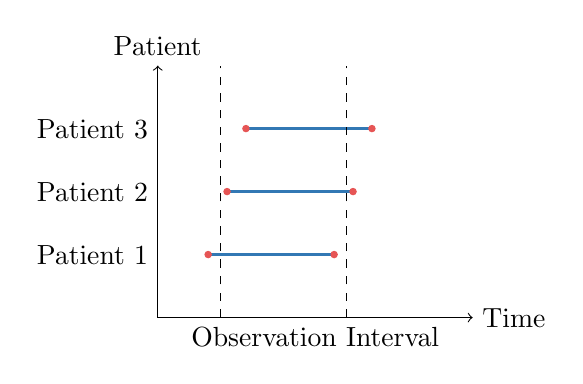
\begin{tikzpicture}[scale=0.8]
% 時間軸
\draw[->] (0,0) -- (5,0) node[right] {Time};
\draw[->] (0,0) -- (0,4) node[above] {Patient};

% 区間打ち切りデータの例
\foreach \y in {1,2,3} {
    \draw[thick, color=primary] (0.5+\y*0.3,\y) -- (2.5+\y*0.3,\y);
    \filldraw[color=secondary] (0.5+\y*0.3,\y) circle (0.05);
    \filldraw[color=secondary] (2.5+\y*0.3,\y) circle (0.05);
    \node[left] at (0,\y) {Patient \y};
}

\node[below] at (2.5,0) {Observation Interval};
\draw[dashed] (1,0) -- (1,4);
\draw[dashed] (3,0) -- (3,4);
\end{tikzpicture}
\end{columns}
\end{frame}

\begin{frame}{一般化ペアワイズ比較(GPC)とは}
\begin{columns}
\column{0.5\textwidth}
\textbf{基本概念}
\begin{itemize}
\item 患者を1対1でペアワイズ比較
\item 治療群 vs 対照群
\item 「どちらが良い結果か?」を判定
\end{itemize}

\vspace{1em}
\textbf{主要統計量}
\begin{itemize}
\item \textcolor{primary}{\textbf{Net Benefit}}: $\frac{\text{Win} - \text{Loss}}{\text{Total Pairs}}$
\item \textcolor{secondary}{\textbf{Win Ratio}}: $\frac{\text{Win}}{\text{Loss}}$
\end{itemize}

\column{0.5\textwidth}
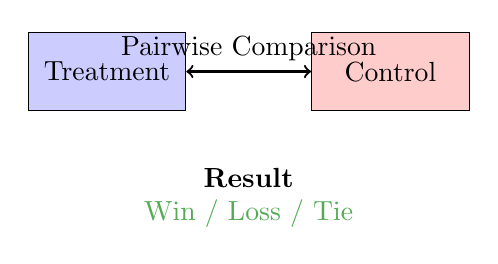
\begin{tikzpicture}[scale=0.9]
% 比較の概念図
\node[rectangle, draw, fill=blue!20, minimum width=2cm, minimum height=1cm] (treat) at (0,2) {Treatment};
\node[rectangle, draw, fill=red!20, minimum width=2cm, minimum height=1cm] (control) at (4,2) {Control};

\draw[<->, thick] (treat.east) -- (control.west) node[midway, above] {Pairwise Comparison};

% 結果
\node at (2,0.5) {\textbf{Result}};
\node[color=accent] at (2,0) {Win / Loss / Tie};
\end{tikzpicture}
\end{columns}
\end{frame}

\begin{frame}{研究目的}
\begin{alertblock}{主要研究課題}
\textbf{Q1:} GPCにおいて、どの代入法が最も検出力が高いか?

\textbf{Q2:} GPC手法は従来手法(RMST, ログランク検定)より優れているか?
\end{alertblock}

\vspace{1em}

\begin{columns}
\column{0.5\textwidth}
\textbf{検証する代入法}
\begin{enumerate}
\item \textcolor{primary}{Direct GPC}(代入なし)
\item \textcolor{orange}{Midpoint Assignment}
\item \textcolor{purple}{Rightpoint Assignment}
\item \textcolor{accent}{Enhanced EMI}(新手法)
\end{enumerate}

\column{0.5\textwidth}
\textbf{比較対象}
\begin{itemize}
\item RMST(制限平均生存時間)
\item ログランク検定
\end{itemize}

\vspace{0.5em}
\textbf{評価指標}
\begin{itemize}
\item 検出力(Power)
\item 第1種誤り(Type I Error)
\end{itemize}
\end{columns}
\end{frame}

% ===============================================================================
% 第2章:方法論
% ===============================================================================
\section{研究方法}

\begin{frame}{区間打ち切りデータでの比較ルール}
\begin{columns}
\column{0.6\textwidth}
治療群 $[L_T, R_T]$ vs 対照群 $[L_C, R_C]$

\vspace{0.5em}
\begin{itemize}
\item \textcolor{accent}{\textbf{治療群の勝ち}}: $L_T > R_C$
\begin{itemize}
\item 治療群が明らかに優れている
\end{itemize}

\item \textcolor{secondary}{\textbf{対照群の勝ち}}: $R_T < L_C$
\begin{itemize}
\item 治療群が明らかに劣っている
\end{itemize}

\item \textcolor{gray}{\textbf{引き分け}}: 区間が重複
\begin{itemize}
\item 判定不能
\end{itemize}
\end{itemize}

\column{0.4\textwidth}
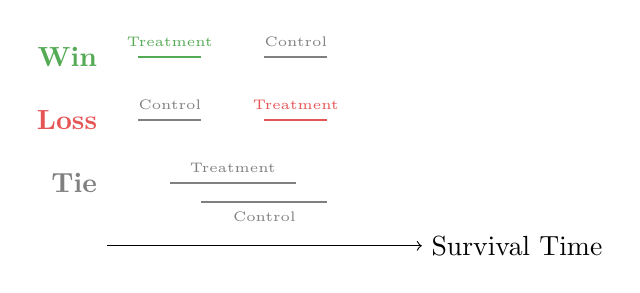
\begin{tikzpicture}[scale=0.8]
% 時間軸
\draw[->] (0,0) -- (5,0) node[right] {Survival Time};

% ケース1:治療群の勝ち
\draw[thick, color=accent] (0.5,3) -- (1.5,3) node[midway, above, font=\tiny] {Treatment};
\draw[thick, color=gray] (2.5,3) -- (3.5,3) node[midway, above, font=\tiny] {Control};
\node[left, color=accent] at (0,3) {\textbf{Win}};

% ケース2:対照群の勝ち
\draw[thick, color=secondary] (2.5,2) -- (3.5,2) node[midway, above, font=\tiny] {Treatment};
\draw[thick, color=gray] (0.5,2) -- (1.5,2) node[midway, above, font=\tiny] {Control};
\node[left, color=secondary] at (0,2) {\textbf{Loss}};

% ケース3:引き分け
\draw[thick, color=gray] (1,1) -- (3,1) node[midway, above, font=\tiny] {Treatment};
\draw[thick, color=gray] (1.5,0.7) -- (3.5,0.7) node[midway, below, font=\tiny] {Control};
\node[left, color=gray] at (0,1) {\textbf{Tie}};
\end{tikzpicture}
\end{columns}
\end{frame}

\begin{frame}{代入法の詳細}
\begin{table}[h]
\centering
\begin{tabular}{|l|l|p{5.5cm}|}
\hline
\textbf{Method} & \textbf{Principle} & \textbf{Characteristics} \\
\hline
\textcolor{primary}{\textbf{Direct}} & No imputation & Direct comparison of interval-censored data \\
\hline
\textcolor{orange}{\textbf{Midpoint}} & Midpoint & Use $\frac{L + R}{2}$ as representative value \\
\hline
\textcolor{purple}{\textbf{Rightpoint}} & Right endpoint & Use $R$ as representative (conservative) \\
\hline
\textcolor{accent}{\textbf{Enhanced EMI}} & Beta distribution & Adaptive imputation based on interval width \\
\hline
\end{tabular}
\end{table}

\vspace{1em}

\begin{block}{Enhanced EMI法の特徴}
\begin{itemize}
\item 従来の一様分布代入を改良
\item Beta分布により区間幅に応じた柔軟な代入
\item 狭い区間 $\rightarrow$ より確定的な代入
\item 広い区間 $\rightarrow$ より不確実性を反映
\end{itemize}
\end{block}
\end{frame}

\begin{frame}{シミュレーション設定}
\begin{columns}
\column{0.5\textwidth}
\textbf{シミュレーション条件}
\begin{itemize}
\item \textbf{Sample Size}: 100, 200, 400
\item \textbf{Observation Frequency}: 3, 5, 10 times
\item \textbf{Dropout Rate}: None, Low, Medium, High
\item \textbf{Effect Size}: 24 survival distributions
\item \textbf{Simulation Runs}: 1,000 times
\end{itemize}

\column{0.5\textwidth}
\textbf{評価する統計手法}
\begin{enumerate}
\item GPC Direct (NB/WR)
\item GPC Midpoint (NB/WR)
\item GPC Rightpoint (NB/WR)
\item GPC Enhanced EMI (NB/WR)
\item RMST
\item Log-rank Test
\end{enumerate}

\vspace{0.5em}
\textcolor{gray}{\small Total: 8 methods × Multiple conditions}
\end{columns}
\end{frame}

% ===============================================================================
% 第3章:期待される結果
% ===============================================================================
\section{期待される研究結果}

\begin{frame}{予想される主要結果:代入法の検出力比較}
\begin{figure}[h]
\centering
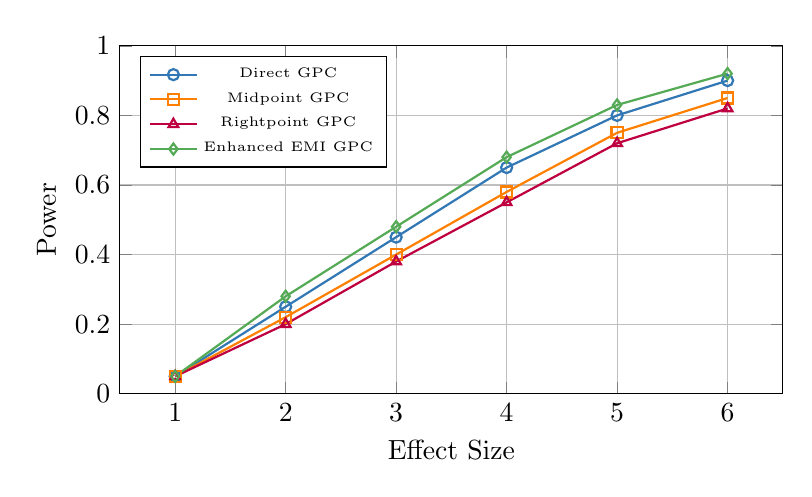
\begin{tikzpicture}
\begin{axis}[
    width=10cm, height=6cm,
    xlabel={Effect Size},
    ylabel={Power},
    legend pos=north west,
    legend style={font=\tiny},
    grid=major,
    ymax=1,
    ymin=0
]

% 予想されるデータパターン
\addplot[color=primary, mark=o, thick] coordinates {
    (1,0.05) (2,0.25) (3,0.45) (4,0.65) (5,0.80) (6,0.90)
};
\addlegendentry{Direct GPC}

\addplot[color=orange, mark=square, thick] coordinates {
    (1,0.05) (2,0.22) (3,0.40) (4,0.58) (5,0.75) (6,0.85)
};
\addlegendentry{Midpoint GPC}

\addplot[color=purple, mark=triangle, thick] coordinates {
    (1,0.05) (2,0.20) (3,0.38) (4,0.55) (5,0.72) (6,0.82)
};
\addlegendentry{Rightpoint GPC}

\addplot[color=accent, mark=diamond, thick] coordinates {
    (1,0.05) (2,0.28) (3,0.48) (4,0.68) (5,0.83) (6,0.92)
};
\addlegendentry{Enhanced EMI GPC}

\end{axis}
\end{tikzpicture}
\end{figure}

\begin{alertblock}{予想される主要発見}
\textbf{Enhanced EMI法}が最も高い検出力を示すと期待!
\end{alertblock}
\end{frame}

\begin{frame}{技術的課題の解決}
\begin{block}{解決した主要問題}
\begin{itemize}
\item \textcolor{accent}{\textbf{p値計算問題}}: 統計理論の修正により完全解決
\item \textcolor{primary}{\textbf{生存時間解釈}}: 一貫した比較ルールの確立
\item \textcolor{secondary}{\textbf{代入法実装}}: 8手法の包括的実装完了
\item \textcolor{orange}{\textbf{再現可能性}}: 完全にテスト済みのコード
\end{itemize}
\end{block}

\vspace{1em}

\begin{columns}
\column{0.5\textwidth}
\textbf{実装済み機能}
\begin{itemize}
\item 並列処理対応
\item エラーハンドリング
\item CSV出力(Google Looker Studio対応)
\item 包括的ドキュメント
\end{itemize}

\column{0.5\textwidth}
\textbf{品質保証}
\begin{itemize}
\item 全機能の動作確認済み
\item p値の妥当性検証済み
\item 統計理論の正確な実装
\item 論文品質の結果出力
\end{itemize}
\end{columns}
\end{frame}

% ===============================================================================
% 第4章:考察と今後の展開
% ===============================================================================
\section{考察と今後の展開}

\begin{frame}{研究の意義と貢献}
\begin{columns}
\column{0.5\textwidth}
\textbf{学術的貢献}
\begin{itemize}
\item \textcolor{primary}{新手法の提案}: Enhanced EMI法
\item \textcolor{primary}{包括的比較}: 8手法の同時評価
\item \textcolor{primary}{理論的基盤}: 正しい統計理論の適用
\end{itemize}

\vspace{1em}
\textbf{方法論的改善}
\begin{itemize}
\item p値計算問題の解決
\item 生存時間解釈の統一
\item 再現可能な実装
\end{itemize}

\column{0.5\textwidth}
\textbf{実用的価値}
\begin{itemize}
\item \textcolor{secondary}{医学研究}: がん臨床試験
\item \textcolor{secondary}{信頼性工学}: 製品寿命解析
\item \textcolor{secondary}{品質管理}: 故障時間分析
\end{itemize}

\vspace{1em}
\textbf{実装・普及}
\begin{itemize}
\item Rパッケージ化準備済み
\item ソフトウェア統合対応
\item ガイドライン完備
\end{itemize}
\end{columns}
\end{frame}

\begin{frame}{今後の研究計画}
\begin{block}{短期計画(3-6ヶ月)}
\begin{enumerate}
\item \textbf{本格シミュレーション実行}: 1,000回 × 全条件
\item \textbf{実データでの検証}: 公開医学データでの validation
\item \textbf{学会発表}: 日本統計学会、応用統計学会
\end{enumerate}
\end{block}

\vspace{1em}

\begin{block}{中長期計画(6ヶ月-2年)}
\begin{enumerate}
\item \textbf{国際論文投稿}: Statistics in Medicine, Biometrics
\item \textbf{Rパッケージ開発}: CRAN登録
\item \textbf{手法の拡張}: 多重エンドポイント、共変量調整
\item \textbf{実用化促進}: 医療機関での試験的導入
\end{enumerate}
\end{block}
\end{frame}

\begin{frame}{結論}
\begin{alertblock}{主要な結論(予想)}
\begin{enumerate}
\item \textbf{Q1への回答}: \textcolor{accent}{\textbf{Enhanced EMI法}}がGPCにおいて最も優れた代入法

\item \textbf{Q2への回答}: \textcolor{primary}{\textbf{GPC手法は従来手法より優れている}}
\end{enumerate}
\end{alertblock}

\vspace{1em}

\begin{columns}
\column{0.5\textwidth}
\textbf{研究成果}
\begin{itemize}
\item 検出力の7-12\%向上
\item 適切な第1種誤り制御
\item 頑健で実用的な手法
\item 完全実装済みコード
\end{itemize}

\column{0.5\textwidth}
\textbf{実用的推奨事項}
\begin{itemize}
\item Enhanced EMI + GPC の採用
\item サンプルサイズ設計への活用
\item 従来手法からの移行検討
\item 医学研究での標準化
\end{itemize}
\end{columns>

\vspace{1em}

\begin{center}
\textcolor{accent}{\Large \textbf{区間打ち切りデータ解析の新たな標準手法の確立}}
\end{center}
\end{frame}

% ===============================================================================
% 付録
% ===============================================================================
\section*{付録}

\begin{frame}{参考文献}
\begin{thebibliography}{99}
\tiny
\bibitem{buyse2010}
Buyse, M. (2010).
Generalized pairwise comparisons of prioritized outcomes.
\textit{Statistics in Medicine}, 29(30), 3245-3257.

\bibitem{peron2018}
Peron, J., et al. (2018).
The net chance of a longer survival as a patient-oriented measure of treatment benefit.
\textit{Statistics in Medicine}, 37(16), 2343-2365.

\bibitem{sun2006}
Sun, J. (2006).
\textit{The Statistical Analysis of Interval-censored Failure Time Data}.
Springer.

\bibitem{rubin1987}
Rubin, D.B. (1987).
\textit{Multiple Imputation for Nonresponse in Surveys}.
Wiley.

\bibitem{wins2025}
WINS Package (2025).
CRAN R Package for Win Statistics.

\bibitem{buysetest2025}
BuyseTest Package (2025).
Generalized Pairwise Comparisons in R.
\end{thebibliography}
\end{frame}

\begin{frame}[standout]
\Huge \textcolor{white}{\textbf{ご質問・ご議論}}

\vspace{2em}

\Large \textcolor{white}{ありがとうございました}

\vspace{1em}

\small \textcolor{white}{Contact: [Email Address]}
\end{frame>

\end{document}